\documentclass[a4paper,12pt,fleqn]{article}
\usepackage{amsmath, amssymb}
\usepackage{bbm}
\usepackage{enumitem}
\usepackage{array}
\usepackage{fancyhdr}
\usepackage{graphicx}
\usepackage{color}

% Insert your course information here %%%%%%%%%%%%%%%%%%%%%%%%%%%%%%%%%%

\newcommand{\titlehd}{Computational Data Analysis}
\newcommand{\examtype}{\bf Final Exam}
\newcommand{\examdate}{Spring 2020}
\newcommand{\examcode}{ISYE 6740}
%\newcommand{\writetime}{}
\newcommand{\total}{100}
\newcommand{\lastwords}{End of Examination}

%%%%%%%%%%%%%%%%%%%%%%%%%%%%%%%%%%%%%%%%%%%%%%%%%%%%

%\setcounter{MaxMatrixCols}{10}
\newtheorem{theorem}{Theorem}
\newtheorem{acknowledgement}[theorem]{Acknowledgement}
\newtheorem{algorithm}[theorem]{Algorithm}
\newtheorem{axiom}[theorem]{Axiom}
\newtheorem{case}[theorem]{Case}
\newtheorem{claim}[theorem]{Claim}
\newtheorem{conclusion}[theorem]{Conclusion}
\newtheorem{condition}[theorem]{Condition}
\newtheorem{conjecture}[theorem]{Conjecture}
\newtheorem{corollary}[theorem]{Corollary}
\newtheorem{criterion}[theorem]{Criterion}
\newtheorem{definition}[theorem]{Definition}
\newtheorem{example}[theorem]{Example}
\newtheorem{exercise}[theorem]{Exercise}
\newtheorem{lemma}[theorem]{Lemma}
\newtheorem{notation}[theorem]{Notation}
\newtheorem{problem}[theorem]{Problem}
\newtheorem{proposition}[theorem]{Proposition}
\newtheorem{remark}[theorem]{Remark}
\newtheorem{solution}[theorem]{Solution}
\newtheorem{summary}[theorem]{Summary}
\newenvironment{proof}[1][Proof]{\noindent\textbf{#1.} }{\ \rule{0.5em}{0.5em}}
\newcounter{questionnumber}
\stepcounter{questionnumber}

\newcommand{\questionnumber}{\noindent \arabic{questionnumber}\stepcounter{questionnumber})~~}
\newcommand{\truefalse}[1]{\questionnumber #1\\True~~~~~~~~False\\Explanation if False:\\ \vspace{3cm}}
\newcommand{\norm}[1]{\|#1\|}
\newcommand{\RR}{\mathbb{R}}
\newcommand{\argmin}{\mathop{\arg\min}}

% ANU Exams Office mandated margins and footer style
\setlength{\topmargin}{0cm}
\setlength{\textheight}{9.25in}
\setlength{\oddsidemargin}{0.0in}
\setlength{\evensidemargin}{0.0in}
\setlength{\textwidth}{16cm}
\pagestyle{fancy}
\lhead{} 
\chead{} 
\rhead{} 
\lfoot{} 
\cfoot{\footnotesize{Page \thepage \ of \pageref{finalpage} -- \titlehd \ (\examcode)}} 
\rfoot{} 

% DEPRECATED: ANU Exams Office mandated margins and footer style
%\setlength{\topmargin}{0cm}
%\setlength{\textheight}{9.25in}
%\setlength{\oddsidemargin}{0.0in}
%\setlength{\evensidemargin}{0.0in}
%\setlength{\textwidth}{16cm}
%\pagestyle{fancy}
%\lhead{} %left of the header
%\chead{} %center of the header
%\rhead{} %right of the header
%\lfoot{} %left of the footer
%\cfoot{} %center of the footer
%\rfoot{Page \ \thepage \ of \ \pageref{finalpage} \\
%       \texttt{\examcode}} %Print the page number in the right footer

\renewcommand{\headrulewidth}{0pt} %Do not print a rule below the header
\renewcommand{\footrulewidth}{0pt}


\begin{document}

% Title page
\begin{center}
\large\textbf{\titlehd}
\end{center}

\begin{center}
\large\textbf{\examcode}
\end{center}

\begin{center}
\textit{ \examtype -- \examdate}
\end{center}

%\begin{center}
%\textit{Writing Time: \writetime}
%\end{center}

\begin{center}
\textit{Total Score: \total}
\end{center}

\vspace{2cm}
If you think a question is unclear or multiple answers are reasonable, please write a brief explanation of your answer,
 to be safe. Also, show your work if you want wrong answers to have a chance at some credit: it lets us see how much you understood.\\\\
(Please sign the honor code below.) I will obey GT Honor Code. I have neither given nor received any unauthorized aid on this exam. I understand that the work contained herein is wholly my own without the aim from a 3rd person. %I understand that violation of these rules, including using an authorized aid or copying from another person,may result in my receiving a 0 on this exam.
\\\\

\textcolor{red}{\bf
You are only required to finish ONE of the Programming Questions, i.e., please pick either Question 8 or Question 9 to work on. If you decide to try both, you will receive BONUS points (please indicate which question you would like to use as BONUS).
}\\\\

\textcolor{red}{\bf Please submit a zip folder, with your final answers (in pdf file format) and code for your Program Question(s).}


\begin{table}[h]
\centering
\begin{tabular}{m{8cm}}
\\
\\
\vspace{0.2in}
\textbf{Name}: 
\vspace{0.7in}

\textbf{GT ID:}
\vspace{0.7in}


\textbf{GT Account:}
\end{tabular}
\end{table}
\newpage

\begin{table}[h]
\centering
\begin{tabular}{| m{6cm} | m{6cm} |}
\hline
\vspace{0.5cm}
Question 1 [10 points] & \\
\vspace{0.5cm} &\vspace{0.5cm}\\
\hline
\vspace{0.5cm}
Question 2 [10 points] & \\
\vspace{0.5cm} &\vspace{0.5cm}\\
\hline
\vspace{0.5cm}
Question 3 [10 points] & \\
\vspace{0.5cm} &\vspace{0.5cm}\\
\hline
\vspace{0.5cm}
Question 4 [10 points] &  \\
\vspace{0.5cm} &\vspace{0.5cm}\\
\hline
\vspace{0.5cm}
Question 5 [15 points] & \\
\vspace{0.5cm} &\vspace{0.5cm}\\\hline
\vspace{0.5cm}
Question 6 [15 points] & \\
\vspace{0.5cm} &\vspace{0.5cm}\\\hline
\vspace{0.5cm}
Question 7 [10 points] & \\
\vspace{0.5cm} &\vspace{0.5cm}\\\hline

\vspace{0.5cm}
Question 8 [20 points] & \\
\vspace{0.5cm} &\vspace{0.5cm}\\\hline

\vspace{0.5cm}
Question 9 [20 points] & \\
\vspace{0.5cm} &\vspace{0.5cm}\\\hline



\hline
\end{tabular}
\end{table}


\clearpage

\section{\bf $K$-means (10 points)}

Given $m = 5$ data points configuration in Figure 1. Assume $K = 2$ and use Manhattan distance (a.k.a. the $\ell_1$ distance: given two 2-dimensional points $(x_1, y_1)$ and $(x_2, y_2)$, their distance is $|x_1 - x_2| + |y_1 - y_2|$).  Assuming the initialization of centroid as shown, after one iteration of k-means algorithm, answer the following questions. 

\begin{enumerate}
\item[(a)] (3 points) Show the cluster assignment;
\item[(b)] (4 points) Show the location of the new center;
\item[(c)] (3 points) Will it terminate in one step?
\end{enumerate}

\begin{figure}[h!]
\begin{center}
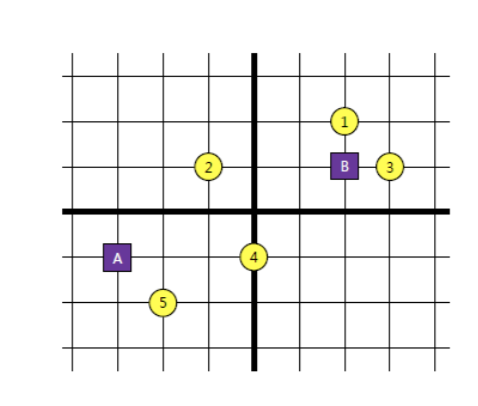
\includegraphics[width = 0.5\textwidth]{./fig/points.png}
\end{center}
\caption{Question 1.}
\end{figure}


\clearpage
\section{Clustering [10 pts]}


\begin{enumerate}

\item (3 points) Explain what is the difference between $K$-means and spectral clustering? 

\vspace{1.5in}


\item (3 points) What is in common, and what is the main difference between spectral clustering and PCA?

\vspace{1.5in}

\item (4 points) For the following data (two moons), give one method that will successfully separate the two moons? Explain your rationale. 

\begin{center}
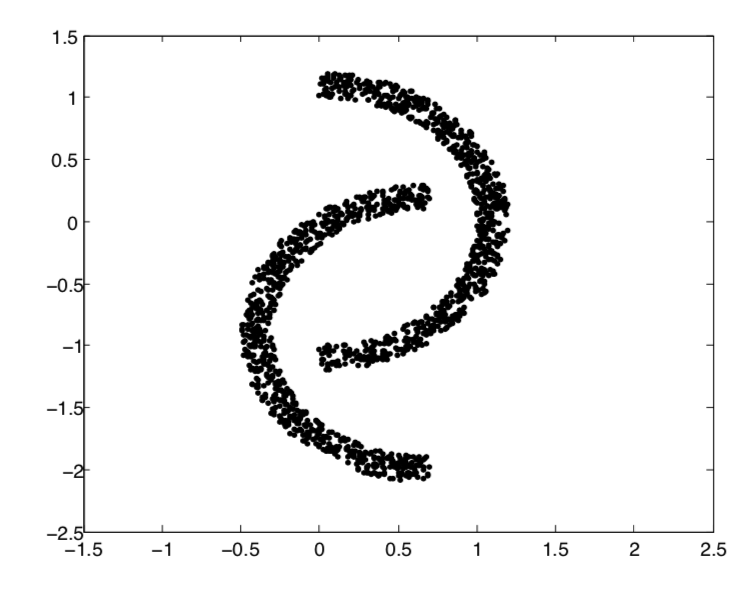
\includegraphics[width = 0.5\textwidth]{./fig/moon}
\end{center}

\end{enumerate}

\vspace{1.5in}
%\clearpage
\section{Principal Component Analysis (10 pts)}

\textcolor{blue}{Suppose we have 4 points in 3-dimensional Euclidean space, namely $(1, 0, 0.5)$, $(6, 14, 3)$, $(11, 28, 5.5)$, and $(7, 21, 3.5)$.}

\vspace{.1in}

(a) (3 points) Find the first principal direction. First, write down the data matrix and make sure you fill in numbers specific for this problem. Then explain how to find the first principal direction and what is the optimization problem you need to solve? Find the first principal direction either by calculation in hand, or using program or software - report  the first principal direction you found.


\vspace{4cm}
(b) (2 points) What are the first principle components, for each of the data points?


\vspace{4cm}
(c) (2 points) When we reduce the dimensionality from 3 to 1 based on the principal direction you found in (a), what is the remaining variance in the data?


\vspace{4cm}
(d) (3 points) You are given the following 2-D datasets, approximately draw the first and second principal directional on each plot.

\begin{figure}[h!] 
        \begin{center}
        \begin{tabular}{cc}
                   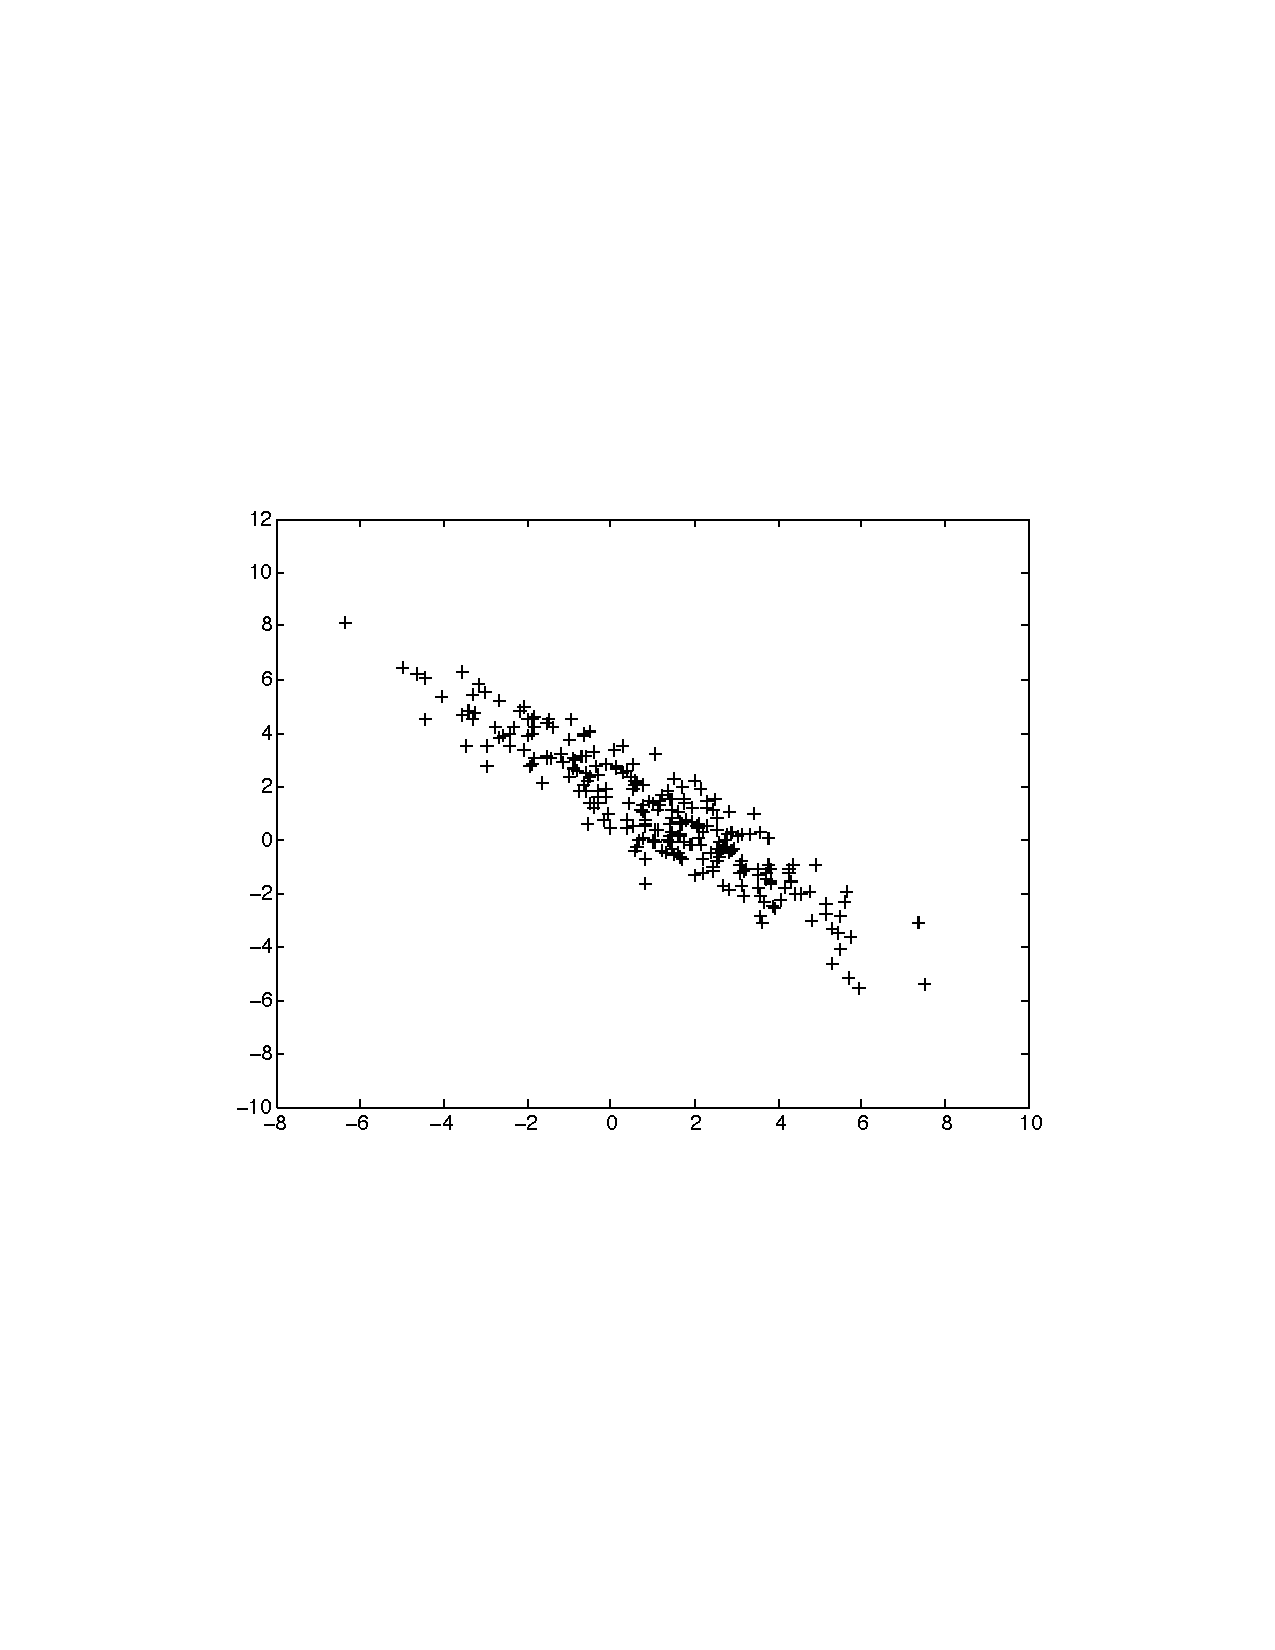
\includegraphics[
                width = 5.5 cm,height=4.5cm
                            ]{./fig/PCA1} 
                 &
                    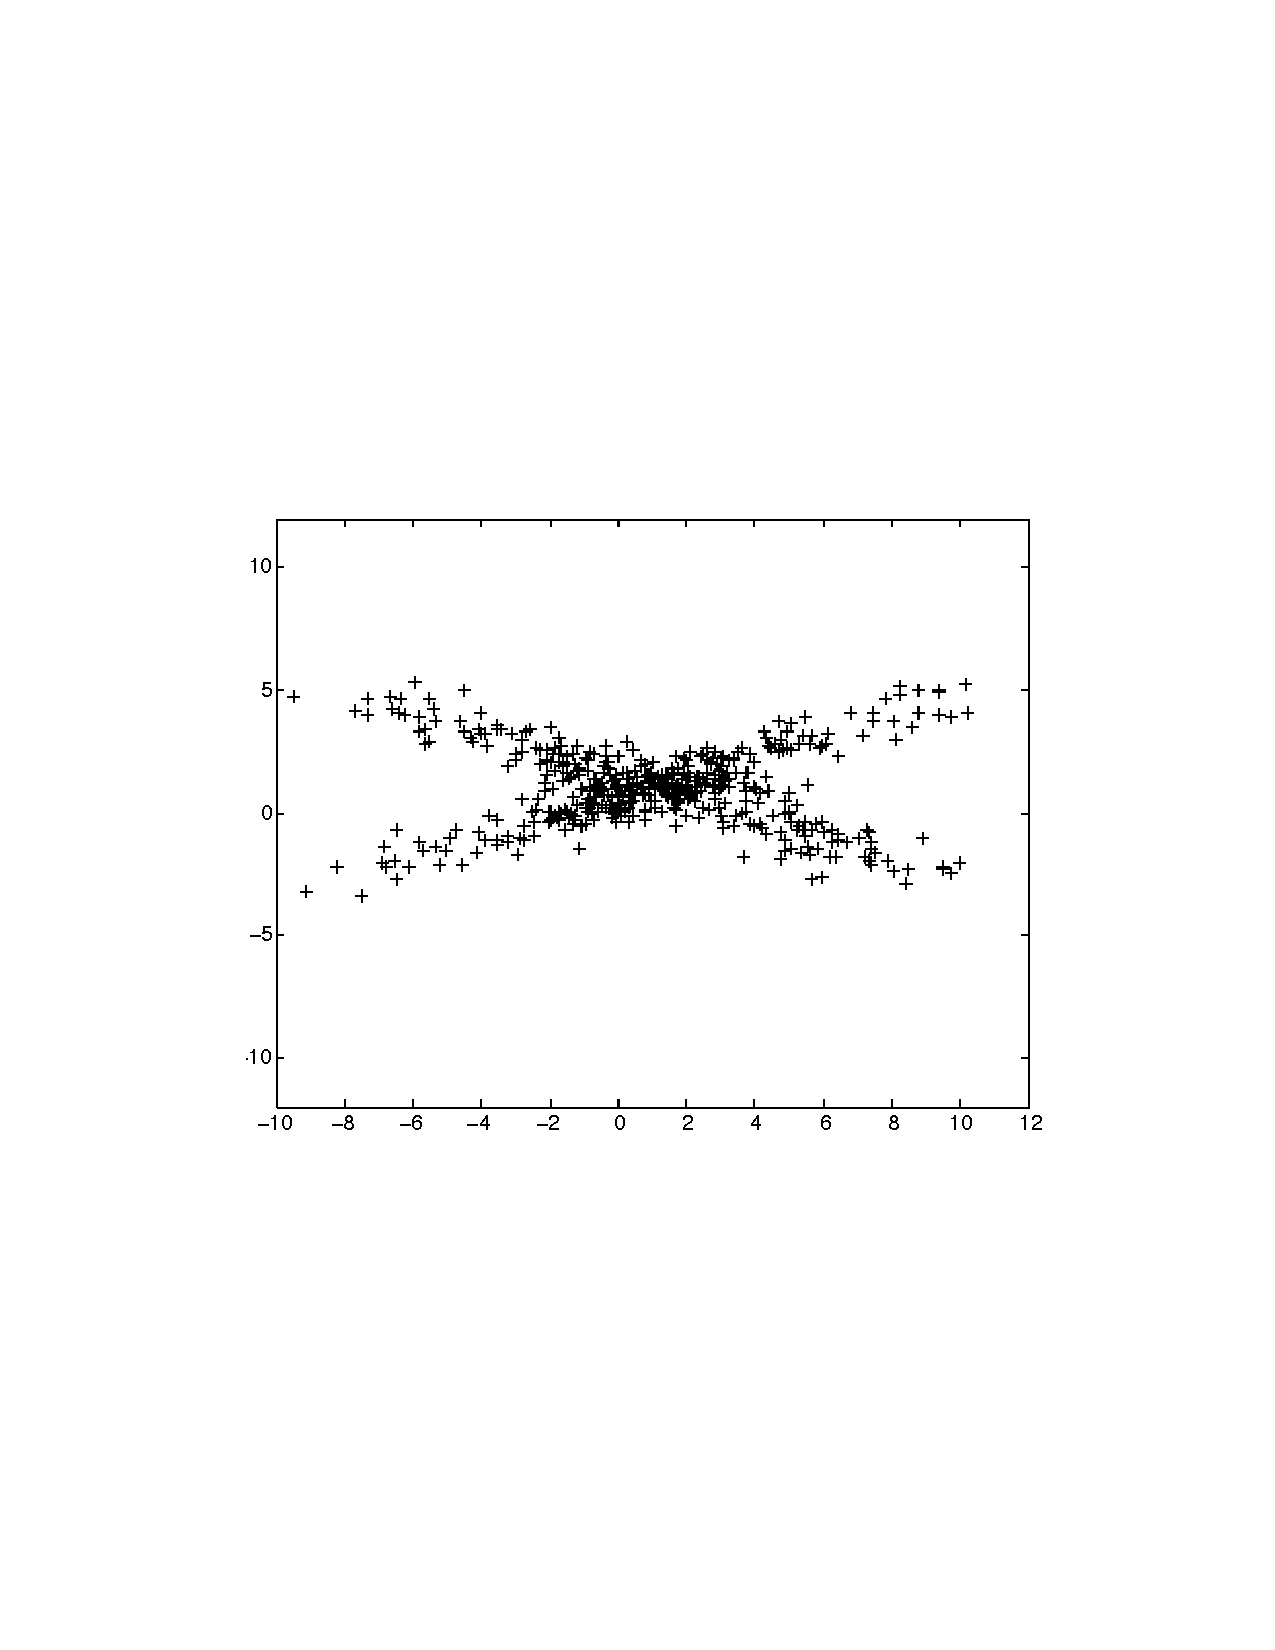
\includegraphics[width = 5.5cm,height=4.5cm
                    ]   {./fig/PCA2} \\
                    (a)&(b)
                    \end{tabular}
                    \end{center}
 \end{figure}

\clearpage
\section{Classification [10 points]}

\begin{enumerate}
\item (5 points) List all methods below which can be used for classification:

(a) AdaBoost (b) Decision Trees (c) EM and Gaussian Mixture (d) Histogram (e) $K$-nearest neighbors (f) $K$-means (g) Kernel density estimation 
(h) Linear Regression (i) Logistic Regression (j) Naive Bayes. 



\vspace{1.3in}

\item (5 points) Which of the decision boundaries below correspond to (a) Random Forest, (b) Decision Tree, (c) SVM. Explain your reasons  to fully justify your answers. 
%
\begin{center}
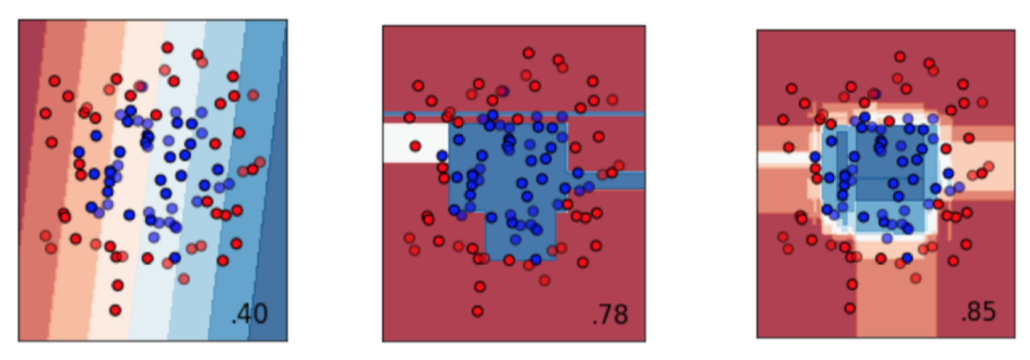
\includegraphics[width = 0.6\textwidth]{./fig/decision}
\end{center}

%\vspace{1in}
%
%\item (3 points) Is the following statement true / false: ``In the AdaBoost algorithm, the weights on all the
%misclassified points will go up by the same multiplicative factor.'' Explain your reason.

\end{enumerate}


\clearpage
\section{SVM [15 points]}

Suppose we only have four training examples in two dimensions as shown in Fig. The positive samples at $x_1 = (0, 0)$, $x_2 = (2, 2)$ and negative samples at $x_3 = (h, 1)$ and $x_4 = (0, 3)$. 
%
\begin{center}
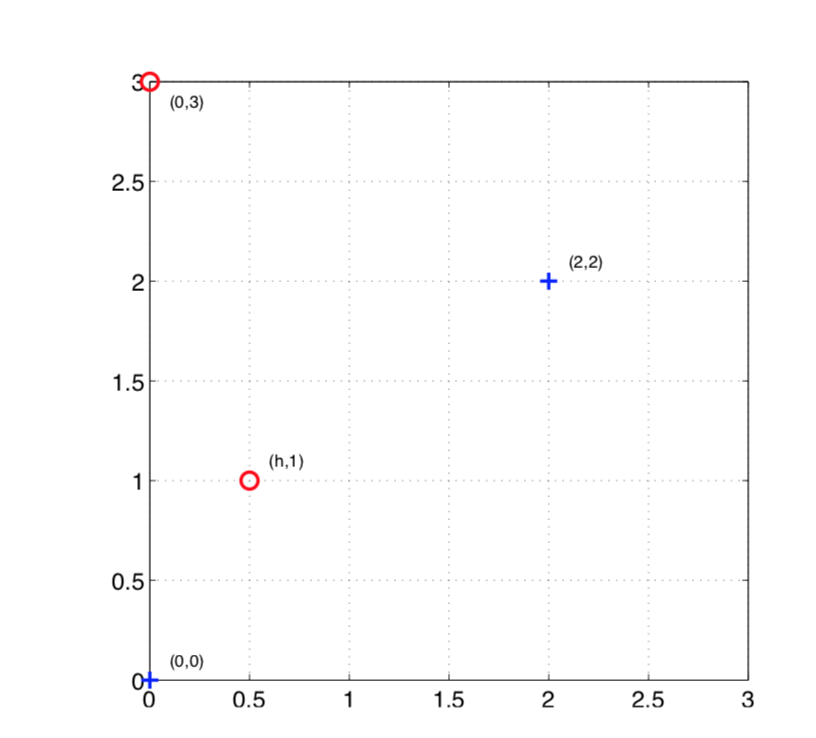
\includegraphics[width = 0.5\textwidth]{./fig/svm}
\end{center}

\begin{enumerate}
\item (5 points) For what range of parameter value $h > 0$ be so that the training points are still linearly separable?

\vspace{1in}

\item (5 points) Does the orientation of the maximum margin decision boundary change as a function of $h$ when the points are separable?

\vspace{1.5in}

\item (5 points) Explain why only the data points on the ``margin'' will contribute to the decision boundary?
\end{enumerate}



\clearpage

\section{Boosting algorithms [15 points]}
In this problem, we test your understanding of AdaBoost algorithm. The figure shows a dataset of 8 points, equally divided among the two classes (positive and negative). The figure also shows a particular choice of decision stump $h_1$ picked by Adaboost in the first iteration. 

\begin{figure}[ht]%{0.5\textwidth}
  \begin{center}
    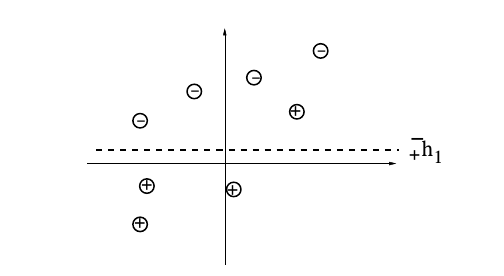
\includegraphics[width=0.7\columnwidth, trim = 0 100 0 0]{./fig/adaboost.png}
  \end{center}
\end{figure}

\vspace{2cm}

\begin{enumerate}
\item[(a)] (6 points) Explain the weights $D_2(i)$ for each sample after the first iteration. You can explain by drawing figures similar to what we have in class. 

\vspace{3cm}

\item[(b)] (6 points) Calculate the weight $\alpha_1$ assigned to $h_1$ by Adaboost? (Note that initial weights of all the data points are equal, $D_1(i) = 1/8, \forall i$ ). 
\vspace{3cm}


\item[(c)] \textbf{[True/False]} (3 points) The votes $\alpha_i$ assigned to weak classifiers in boosting generally changes monotonically as the algorithm proceeds. %, because the weighted training error of the weak classifiers tend tends to go up.



\end{enumerate}


\clearpage

\section{Variable section [10 points]}

Suppose we have data $\{x_i, y_i\}$, $i = 1, \ldots, m$, where $x_i \in \mathbb R^p$ corresponds to $p$ features.


\begin{enumerate}
\item (3 points) Write down the optimization problem we solve with Ridge Regression and Lasso. Make sure you explain your notations: which are the decision variables, and which are data. 

\vspace{1.5in}


\item (3 points) Which of the solution paths below corresponds to Ridge regression and which corresponds to Lasso?
%
\begin{center}
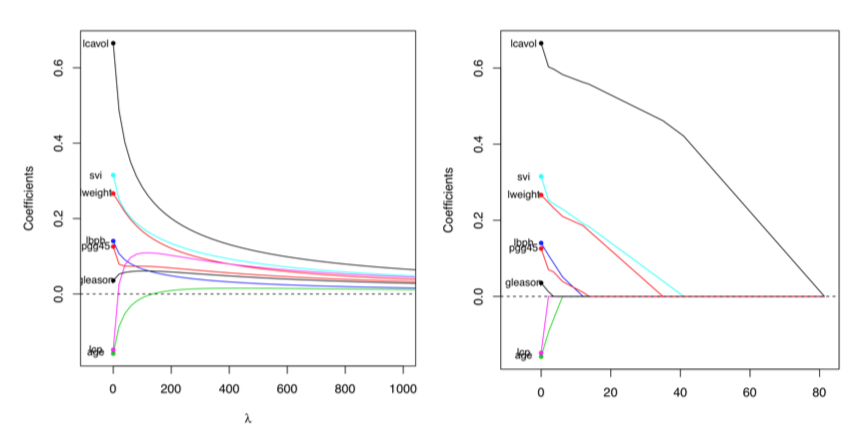
\includegraphics[width = 0.8\textwidth]{./fig/path}
\end{center}

\vspace{0.3in}

\item (2 points) Explain what's the difference between Lasso and Ridge regression. We need Lasso for what setting?

\vspace{0.9in}

\item (2 points) Explain how to tune the regularization parameters for Lasso and Ridge regression (hint: CV). 

\vspace{1.5in}

\end{enumerate}


\clearpage 

\textcolor{red}{\bf
You are only required to finish ONE of the Programming Questions, i.e., please pick either Question 8 or Question 9 to work on. If you decide to try both, you will receive BONUS points (please indicate which question you would like to use as BONUS).
}

\textcolor{red}{\bf Please submit a zip folder, with your final answers (in pdf file format) and code for your Program Question(s).}

\section{PCA for face recognition (20 points)}

This question is a simplified illustration of using PCA for face recognition using a subset of data from the famous Yale Face dataset. 

 {\bf Remark:} you have to perform downsampling of the image by a factor of 4 to turn them into a lower resolution image before we do anything. 


\begin{enumerate}
\item 
(10 points) 
First, given a set of images for each person, we generate the so-called eigenface using these images. The procedure to obtain eigenface is explained as follows. 
%
Given $n$ images of the {\it same person} denoted by $x_1, \ldots, x_n$. Each image originally is a matrix. We vectorize each image to form the vector $x_i \in \mathbb R^p$. Now form a matrix
\[
X = [x_1, \ldots, x_n] \in \mathbb R^{p\times n}.
\]

Extract the largest $k$ eigenvector of the data matrix $X^\top X$, denoted as $u_1, u_2,  \ldots, u_k$. The eigenfaces correspond to the projections $\textsf{eigenface}_i = X u_i$, $i = 1, \ldots, k$.

Perform analysis on the Yale face dataset for subject 14 and subject 01, respectively, using all the images EXCEPT for the two images named \textsf{subject01-test.gif} and \textsf{subject14-test.gif}. {\bf Plot the top 6 eigenfaces for each subject.} When visualizing, you have to reshape the eigenvectors into images with the same dimension as the original images. 

{\bf What is the interpretation of the top 6 eigenfaces?}

\item (10 points) Now we will perform a face recognition task. 

For doing face recognition through PCA we proceed as follows. Given the test image \textsf{subject01-test.gif} and \textsf{subject14-test.gif}, we vectorize each image. Take the top eigenfaces of Subject 1 and Subject 14, respectively, project the 2 vectorized test images using the vectorized eigenfaces to obtain scores, respectively. \\(Hint: use $\textsf{(eigenface}_1)^\top \textsf{(test image)}$ )

Report four scores: (1) projecting test image of Subject 1 using eigenface of Subject 1; (2) projecting test image of Subject 1 using eigenface of Subject 14; (3) projecting test image of Subject 14 using eigenface of Subject 1; (4) projecting test image of Subject 14 using eigenface of Subject 14. 

Explain whether or not (and how) can you recognize the faces of the test images using these scores. 


\end{enumerate}


\clearpage
\textcolor{red}{\bf
You are only required to finish ONE of the Programming Questions, i.e., please pick either Question 8 or Question 9 to work on. If you decide to try both, you will receive BONUS points (please indicate which question you would like to use as BONUS).
}

\textcolor{red}{\bf Please submit a zip folder, with your final answers (in pdf file format) and code for your Program Question(s).}

\section{Programming: Bayes and KNN classifier [20 points]}


In this programming assignment, you are going to apply the Bayes Classifier to handwritten digits classification problem. Here, we use the binary 0/1 loss for binary classification, i.e., you will calculate the miss-classification rate as a performance metric. To ease your implementation, we selected two categories from USPS dataset in \textsf{usps-2cls.mat} (or \textsf{usps-2cls.dat}, \textsf{usps-2cls.csv}).

\begin{enumerate}
\item (10 points)
Your first task is implementing the classifier by assuming the covariance matrices for two classes are a diagonal matrix $\Sigma_1$, $\Sigma_ 2$. 

Using slides from ``Classification I'', assuming $P(y=1) = P(y=-1)$ (i.e., the prior distribution for two classes are the same), using Bayes decision rule to write down the decision boundary. (Hint, it should be a quadratic decision boundary.)


Now we will estimate the mean vector and the sample covariance matrices for two classes using the training data (hint: you can use sample mean and sample covariance vector). Report the misclassification rate (error rate) over the training set and over the testing set averaged over the 100 random train/test splits by using different value of splitting ratio $p$. Explain and compare the performance of each classifier.

After implementing these methods, you should evaluate your algorithm on the given set. Repeat 100 times: split the dataset into two parts randomly, use $p$ portion for training and the other $1 - p$ portion for testing. Let $p$ change from 0.1, 0.2, 0.5, 0.8, 0.9.

Please implement the algorithm {\bf from scratch} yourself. Make sure to provide code, results (required above) together with necessary explanations to your results. 

\item (10 points) Now repeat the classification again using $K$-nearest neighbors, for $K = 5, 10, 15, 30$.  Repeat 100 times: split the dataset into two parts randomly, use $p$ portion for training and the other $1 - p$ portion for testing. Let $p$ change from 0.1, 0.2, 0.5, 0.8, 0.9. Report the training error and testing error for each case.

For this part, you may use any package that you like.  Make sure to provide code, results (required above) together with necessary explanations to your results. 

\end{enumerate}


\label{finalpage}

\end{document}